\chapter{Mencius}
\mn{4/10/23}
\section{expérience personnelle}

\begin{singlequote}

Le système scolaire en Chine : on essaye de rentrer dans un bon collège, puis bon lycée, à travers des examens difficiles. Epreuve la plus difficile (Gaokao) pour rentrer à l'université, très sélectif.

Toute notre énergie pour l'examen : pas de temps pour discuter sur la vie. Pression. Une fois dans l'université, plus d'objectifs : le vide. Vivre pour moi même : les \textit{entretiens}, le \textit{mencius}. Une autre vision des études. Perfectibilité de l'homme.  Le confucianisme fait partie de notre héritage mais les personnes n'ont pas le temps de le lire. Ceux qui cherchent voient un héritage très riche.    Bia 
\end{singlequote}


\section{Mencius}

\paragraph{L’époque de Mencius: les Royaumes combattants (481/53-221 AEC)} Pendant cette période, effondrement. Le Roi perd toute son autorité. Après la période de l'antiquité, on a la période de l'Empire qui se termine au 1911. A la fin de l'Antiquité, une effervescence d'idées et de créativité intellectuelles, avec la classe des Shi.

\paragraph{Sept grandes puissances} qui luttent pour l’unification des territoires :
Qin, Qi, Chu, Wei, Zhao, Yan


 \begin{figure}
     \centering
          \caption{Les Etats indépendants avant l’unification de l’empire en 221 avant notre ère}
     \includegraphics{}

     \label{fig:enter-label}
 \end{figure}




\paragraph{bouleversement des ordres}
Alors que lors des royaumes Zhou, seule la famille Zhou a le droit de gouverner, ici on s'ouvre à d'autres personnes. Chaque royaume essaye de s'agrandir.  Les chefs de principautés se nomment rois. 

 

\paragraph{Période de grande effervescence et de liberté intellectuelle}  : « Cent
écoles » s’affrontent et rivalisent

\paragraph{Les shi(h)} Nouvelle classe, en tant que conseillers
des princes. normalement entre la noblesse et les paysans. Dans les rites, des ministres ne savent plus où se mettre. les Shih ont de plus en plus de compétences (attachées à l'étude). Confucius n'était pas le seul.
 


\paragraph{Réformes politiques et militaires} pour se développer dans chaque état. Il faut donc à chaque roi des conseils. Les Shi deviennent conseillers itinérants des rois. Ils voyagent de pays en pays ; Une autonomie face au pouvoir. Les princes les respectent et les considèrent comme des \textit{maitres}. 
\begin{Def}[shi(h) - 士 ]
    Lettrés fonctionnaires pendant la période des royaumes combattants.     Les \textit{Shih}{zi} sont considérés comme des \textit{maîtres} par les princes (on passe d'officiers dans les Royaumes Zhou aux conseillers itinérants). Kong zi, Men Zi, Toa Zi. 
\end{Def}
\paragraph{romanisation de Mencius et Confucius} Avec le néo confucianisme, présent à l'époque de Ricci. Les jésuites romaniseront donc ces deux noms.

\paragraph{période de grande effervescence et de liberté intellectuelle} "cent écoles". On ne cherche pas à restaurer mais le meilleur modèle possible afin de réunir toutes les territoires.

\paragraph{Mencius Maître Meng,}
 Son nom personnel : voiture. Originaire de Lu, patrie de Confucius. Au XIè siècle (néo confucianisme), il devient l'héritier orthodoxe de Confucius.

\subsection{sa pensée}

Attirance des nobles mais n'a pas eu de disciples.
La source presqu'unique, c'est le \textit{Mencius}, rédigé par \textit{Mencius et ses disciples ensemble.} Des passages plus long car Mencisu est en débat avec les autres écoles. 

\subsection{Versions citées :}

Séraphin	COUVREUR	(1835-1919),	consultables	et	téléchargeables	sur	le	site https://www.chineancienne.fr (Œuvre de Meng Tzeu [Mengzi, Mencius])
André LÉVY (trad.), Mencius, Paris : Éditions You-Feng, 2003. Anne CHENG, Histoire de la pensée chinoise, Paris : Seuil, 1997.


\section{textes cités}

\subsection{La nature humaine (xing 性) et la perfectibilité de l’homme}

Confucius a dit simplement que la nature de tous les hommes est semblable. Certains de ces disciples (Gaozi), elle est neutre. Mais chez Mencius, il a développé le thème pour dire que la nature humaine est fondamentalement bonne. 


\begin{singlequote}
    1.	Gaozi dit : « La nature est comme le bois de saule, le sens moral comme tasses et bols. Fabriquer du sens de l’humain et du sens du juste à partir de la nature humaine, c’est comme faire des tasses et des bols à partir du bois de saule. »
Mencius dit : « Seriez-vous capable de fabriquer tasses et bols tout en respectant la nature propre du bois de saule ? En fait, c’est en lui faisant violence que vous en faites tasses et bols. Est-ce à dire que vous ferez aussi violence à l’homme pour en tirer sens de l’humain (zen) et sens du juste ? Si quelque chose doit conduire l’humanité tout entière à considérer ces vertus comme des calamités, ce sont bien vos propos ! » 
 \textit{\small (Mencius, VI A 1-2)
-- traduction d’Anne Cheng, p. 170.}
\end{singlequote}

Goazi pense la nature comme ni bonne ni mauvaises. Mencius continue la métaphore en regardant si on suit la nature du bois ou non. Il ne conclue pas mais il montre ainsi que l'argument de Goazi ne tient pas.


\begin{singlequote}
    2.	Kao tzeu [Gaozi] dit :
    
—	La nature est comme une eau qui tourbillonne. Qu’on lui ouvre une voie vers l’orient, elle coulera vers l’orient ; qu’on lui ouvre une voie vers l’occident, elle coulera vers l’occident. La nature humaine ne discerne pas le bien du mal, de même que l’eau ne discerne pas l’orient de l’occident.


Meng tzeu [Mengzi] dit :

—	L’eau ne met aucune différence, il est vrai, entre l’orient et l’occident ; mais n’en met-elle pas entre le haut et le bas ? La nature de l’homme tend au bien, comme l’eau tend en bas. Tout homme est bon comme l’eau tend toujours à descendre.
« Cependant, si en frappant sur l’eau vous la faites jaillir, elle pourra dépasser la hauteur de votre front ; si vous l’arrêtez dans son cours et la refoulez, vous pourrez la faire demeurer sur une montagne. En cela obéira-t-elle à sa tendance naturelle ? Elle obéira à la force. L’homme peut se déterminer à faire le mal ; alors sa nature souffre violence.
-- traduction de S. Couvreur, Mencius, VI.I.2
\end{singlequote}


Etonnant ces discussions de métaphore. C'est lié à la langue chinoise. \cite{vandermeersch_ce_2019} \textit{ce que la pensée chinoise nous apprend} \sn{Ce que la Chine nous apprend. Sur le langage, la société, l'existence », de Léon Vandermeersch, Gallimard, « Bibliothèque des sciences humaines », 182 p., 19,50 €.}
\begin{singlequote}
    3.	Koung tou tzeu dit à Meng tzeu [Mengzi] :
—	Kao tzeu dit : « La nature de l’homme n’est ni bonne ni mauvaise. » Quelques-uns disent :
« La nature peut servir à faire le bien ou à faire le mal. Ainsi au temps de Wenn wang et de Ou wang\sn{Rois sages zhou, modèles}, le peuple aima la vertu ; sous les règnes de Iou wang et de Li wang\sn{modèle des mauvais rois}, le peuple fut enclin au mal. » D’autres disent : « Les hommes sont, les uns naturellement bons, les autres naturellement mauvais. Ainsi, sous un prince excellent comme Iao, il y eut un homme méchant comme Siang ; d’un père détestable comme Keou seou naquit un grand sage comme Chouenn ; avec un neveu et un souverain comme Tcheou, il y eut des hommes vertueux comme K’i, prince
de Wei, et Pi kan, fils d’un empereur. » Vous dites que la nature de l’homme est bonne. Kao tzeu\sn{Idée qu'il met en avant : on ne peut pas dire si la nature est bonne ou mauvaises} et tous les autres sont donc dans l’erreur.
Meng tzeu répondit :
—	Les tendances de notre nature peuvent toutes servir à faire le bien ; voilà pourquoi je dis que la nature est bonne. Si l’homme fait le mal, on ne doit pas en attribuer la faute à ses facultés naturelles.
Tout homme a des sentiments de compassion pour les malheureux, de pudeur et d’aversion pour le mal, de déférence et de respect pour les autres hommes. Il sait discerner le vrai du faux et le bien du mal. La commisération, c’est la bienveillance. La honte et l’horreur du mal, c’est la justice (cette disposition qui nous porte à traiter les hommes et les choses comme il convient). La déférence et le respect constituent l’urbanité. La vertu par laquelle nous discernons le vrai du faux et le bien du mal, c’est la prudence. La bienveillance, la justice, l’urbanité, la prudence ne nous viennent pas du dehors, comme un métal fondu qu’on verse dans un moule. La nature les a mises en nous. (Mais la plupart des hommes) n’y font pas attention. Aussi dit-on : « Si vous les cherchez, vous les trouverez ; si vous les négligez, vous les perdrez. Parmi les hommes, les uns sont deux fois, cinq fois, un nombre indéfini de fois meilleurs ou pires que les autres, parce que la plupart n’arrivent pas à user pleinement de leurs facultés naturelles pour faire le bien.
Il est dit dans le Cheu King :
Le Ciel donne à tous les hommes avec l’existence les principes constitutifs de leur être et la loi morale. Les hommes, grâce à cette loi, aiment et cultivent la vertu.
Confucius dit : « L’auteur de cette ode ne connaissait-il pas la voie de la vertu ? » Ainsi l’homme reçoit toujours, avec les principes constitutifs de son être, la loi morale ; et parce qu’il a cette loi, il aime et cultive la vertu.
-- traduction de S. Couvreur, Mencius, VI.I.6.

\end{singlequote}

\textit{L'homme subit l'influence des autres.
Mencius parle des tendances. Il évoque les quatre qualités, les 4 germes de la moralité : la bienveillance, la justice, l'urbanité et la prudence. Elle sont innée mais on a du mal à les percevoir. L'homme de bien doit les constater et les développer. Ces germes sont assez subtiles, souvent difficiles à percevoir mais sont en nous. 
}

\begin{singlequote}
    4.	Meng tzeu [Mengzi] dit :
—	Autrefois, sur la Montagne des Bœufs (dans le Ts’ing tcheou fou actuel), les arbres étaient beaux. Parce qu’ils étaient sur la limite du territoire d’une grande principauté, la hache et la cognée les ont coupés. Pouvaient-ils conserver leur beauté ?  Comme la sève continuait à circuler (dans les souches mutilées), et que la pluie et la rosée les humectaient, ils ont poussé des bourgeons et des rejets. Mais les bœufs et les brebis, survenant à leur tour, les ont mangés. Voilà pourquoi cette montagne est si nue. En la voyant toute nue, on s’imagine qu’elle n’a jamais eu d’arbres capables de servir pour les constructions. Est-ce un défaut inhérent à sa nature ?
(N’en est-il pas de même) des sentiments que l’homme reçoit de la nature ? N’a-t-il pas des sentiments de bienveillance et de justice ? Ce qui les lui fait perdre, est comme la hache et la cognée à l’égard des arbres. Si chaque jour il leur porte des coups, peuvent-ils se développer ? Nuit et jour, ils tendent à reprendre des forces. Le matin (après le repos de la nuit, quand l’esprit est calme), les affections et les aversions sont quelque peu telles que l’homme doit les avoir. Mais les actions faites pendant la journée interrompent et étouffent les bons sentiments. Après qu’elles les ont étouffés maintes et maintes fois, l’action réparatrice de la nuit n’est plus suffisante pour les préserver d’un anéantissement complet. Quand l’influence bienfaisante de la nuit ne suffit plus pour les conserver, l’homme diffère à peine des animaux. En le voyant devenu comme un être sans raison, on croirait qu’il n’a jamais eu de bonnes qualités. L’homme est-il tel par nature ? Tout être se développe, s’il trouve ce qui est nécessaire à son entretien ; il périt, s’il en est privé. Confucius disait : « Si vous les tenez ferme, ils se conserveront ; si vous les laissez aller, ils se perdront. Ils vont et viennent sans avoir de temps déterminé. Personne ne connaît le lieu où ils demeurent. » Il disait cela en parlant des sentiments du cœur. 
 \textit{\small -- traduction de S. Couvreur, Mencius, VI.I.8.}

\end{singlequote}

Métaphore de la montagne. La moralité est comme les plantes. Les haches abîment la montagne, force extérieure à la montagne. La nature de la montagne n'est pas d'être nue car il faut ces actions de l'extérieur pour devenir nu. Il faut étudier de façon très précise ce qui sort spontanément de nous. 

\begin{singlequote}
    5.	Mencius dit : « Un paulownia ou un catalpa, pas plus gros que les deux mains réunies, si l’on désire le faire pousser, il n’est personne qui ne sache comment le soigner. Quant à ceux qui ne savent même pas comment s’y prendre, s’il s’agit de leur propre personne, serait-ce parce qu’ils tiennent plus aux jeunes arbres qu’à eux-mêmes ? N’est-ce pas le comble de l’inconscience ? »
-- traduction d’André Lévy, Mencius, VI.A.12., p. 161.
\end{singlequote}
Traduction étonnante. Mencius parle beaucoup de nourrir, yang,养. 




\begin{singlequote}
    6.	Mencius dit : « L’humanité est au cœur de l’homme ; l’équité est son chemin. S’écarter de son chemin et ne plus le suivre, laisser son cœur s’égarer et ne plus savoir le retrouver, quelle pitié ! Quand les chiens ou les poulets s’égarent, on sait comment les retrouver, non pas quand il s’agit du cœur !
Les études n’ont d’autre but que de permettre de retrouver le cœur égaré. »
-- traduction d’André Lévy, Mencius, VI.A.11., p. 160.
\end{singlequote}

Coeur égaré comme les bons sentiments qui se font dominer par ce qui vient négativement de l'extérieur. On a négligé ce qui est dans la bonne nature. L'étude est de retrouver le \textit{coeur égaré}.

\begin{Synthesis}
    Chez Mencius, comme des exercices spirituels, comme Pierre Hadot.
    C'est pour cela qu'il a eu bcp de succès avec le développement du Bouddhisme : "nous avons déjà dans le confucianisme ce qu'annonce le bouddhisme, puis les jésuites".
\end{Synthesis}

La locution « les [vieux] cent noms de famille » bǎi xìng (百姓 ou lao bai xing (老百姓) désigne le peuple.  

\begin{singlequote}
    7.	Hao chen Pou hai (qui était de la principauté de Ts’i) dit à Meng tzeu [Mengzi] :
—	Que faut-il penser de Io tcheng tzeu ?

—	C’est un homme bon, un homme sincère, répondit Meng tzeu.

—	Qu’appelez-vous homme bon, homme sincère ? Meng tzeu répondit :

—	On appelle bon celui qui est digne d’être aimé ; sincère, celui dont la bonté est réelle et véritable ; excellent, celui dont la bonté est parfaite ; grand, celui dont la bonté est parfaite et brille d’un grand éclat ; sage par excellence, celui qui est grand, et pour qui la vertu est devenue comme naturelle ; spirituel, celui dont la sagesse est si grande que personne ne peut la  connaître parfaitement. Io tcheng tzeu a dépassé le premier de ces six degrés ; il n’atteint pas le second, encore moins les quatre autres.
-- traduction de S. Couvreur, Mencius, VII.II.25.
\end{singlequote}

Sous forme de jugement : 
\begin{Def}[les degrés de Mencius]
\begin{enumerate}
    \item Bon, Celui digne être aimé (ce qui est désirable pour tous, du fait de la nature humaine)
    \item sincère / fidèle, celui dont la bonté est réelle et véritable (5ème vertu de Confucius) : adéquation entre la forme et l'essence. Quand ces vertus sont intégralement intériorisés, et non superficiels.   
    \item grand, celui dont la bonté est parfaite et brille d’un grand éclat ; 
    \item sage par excellence, celui qui est grand, et pour qui la vertu est devenue comme naturelle ;    
    \item spirituel, celui dont la sagesse est si grande que personne ne peut la  connaître parfaitement.
\end{enumerate}
 
   
\end{Def}


\begin{singlequote}
   8.	— Maître, dit Koung suenn Tch’eou, permettez-moi de vous demander en quoi vous surpassez Kao tzeu [Gaozi].
   
Meng tzeu répondit :


—	Moi, je comprends les paroles (que j’entends dire) ; j’entretiens (je cultive et règle) parfaitement la sensibilité qui est largement répandue en moi.

—	Permettez-moi de vous demander, dit Koung suenn Tch’eou, ce que vous appelez sensibilité largement répandue.


—	Il est difficile de l’expliquer, répondit Meng tzeu. Son action est très puissante, et s’étend fort loin. Si elle est cultivée comme le demande sa nature, si elle n’est pas lésée, elle étend son action partout sous le ciel. Elle prête secours à la justice et à la raison. Sans elle le corps serait languissant.
Il faut qu’elle soit cultivée par des actes de vertu très fréquents ; ce n’est pas une aide que la vertu puisse enlacer et saisir comme une proie pour un acte isolé. Elle est sans force, lorsqu’un homme, en faisant une action, (sent qu’il agit mal et) n’est pas content de lui-même. Aussi, je dis que Kao tzeu n’a pas connu la vertu, lui qui prétend qu’elle ne réside pas dans l’âme.
(Celui qui désire cultiver et régler sa sensibilité), doit faire des actes de vertu, et ne pas prétendre arriver au terme de ses désirs dans un temps déterminé. Qu’il ne néglige jamais la pratique de la vertu, et ne tente pas de hâter son œuvre (par des moyens peu sages). 
Qu’il n’imite pas certain villageois de Soung. Cet homme, voyant avec peine que sa moisson ne grandissait pas, tira les tiges avec la main (pour les allonger). De retour chez lui, ce nigaud dit aux personnes de sa maison :
« Aujourd’hui je suis très fatigué ; j’ai aidé la moisson à grandir. » Ses fils coururent voir son
travail. Les tiges étaient déjà desséchées. Dans le monde il est peu d’hommes qui ne travaillent pas à faire grandir la moisson par des moyens insensés. Ceux qui s’imaginent que la sensibilité (les passions, les affections de l’âme) sont inutiles, et qui les négligent, ressemblent au laboureur qui laisse les mauvaises herbes croître dans sa moisson. Ceux qui emploient des moyens violents pour en développer plus vite l’énergie, font comme cet insensé qui arracha sa moisson. Leurs efforts ne sont pas seulement inutiles ; ils sont nuisibles.
(Koung suenn Tch’eou dit) :
—	Qu’appelez-vous comprendre les paroles ?
Meng tzeu répondit :
—	Si quelqu’un émet une proposition inexacte, je vois en quoi il est aveuglé (par ses mauvaises inclinations). Si quelqu’un ne met aucun frein à sa langue, je vois dans quels excès il se précipite. Si, quelqu’un dit une parole qui porte au mal, je vois en quoi il s’écarte de la voie de la vertu. Si quelqu’un dit des paroles évasives, je vois ce qui l’embarrasse et l’arrête. Les défauts qui se trahissent dans les paroles d’un homme, ont leur source dans son cœur. Ils nuisent à son plan d’administration. Lorsqu’ils se manifestent dans son plan d’administration, ils nuisent à ses affaires. S’il surgissait encore un grand sage, certainement il approuverait ce que je viens de dire.
\textit{\small -- traduction de S. Couvreur, Mencius, II.I.2. }
\end{singlequote}

\begin{Def}[sensibilité]
    "largement répandue en moi" : difficile à expliquer. \textit{souple}, afflux vital, énergie débordante. 
\end{Def}
C'est lié à la morale. Il y a un aspect esthétique (souple). 
\begin{marginfigure}
\caption{Gao, Gu 高濲 : immortels}
    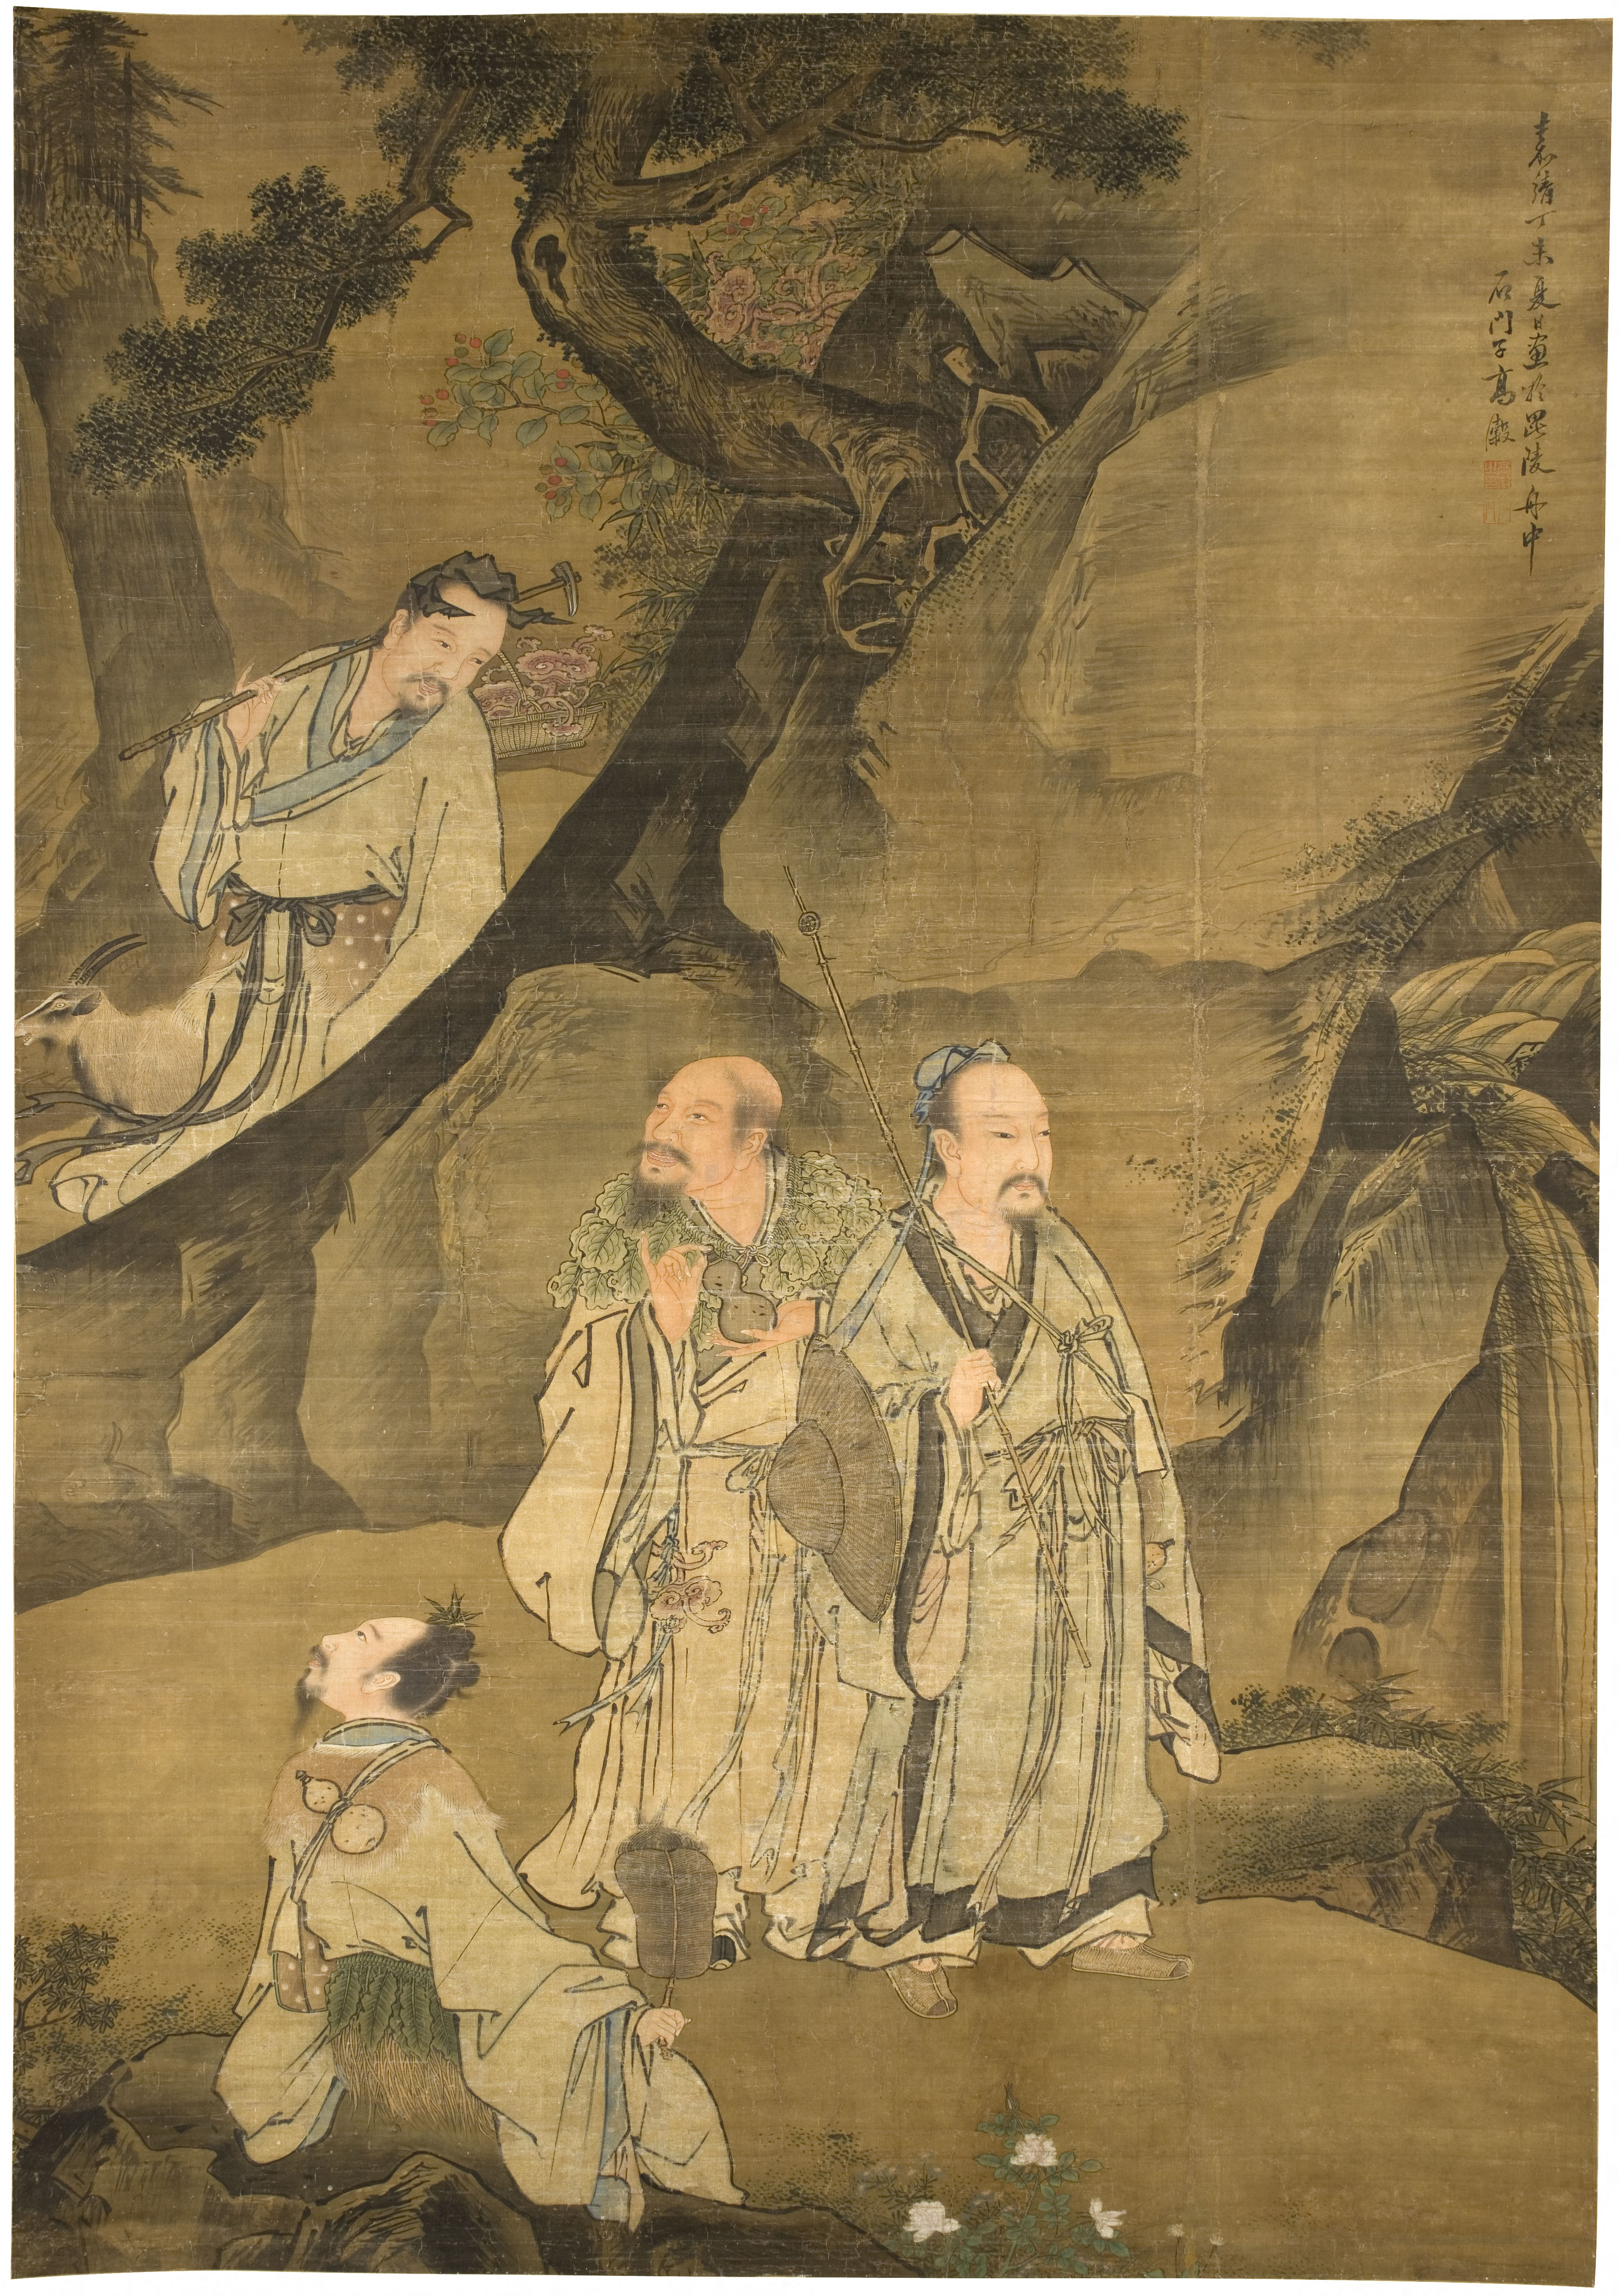
\includegraphics[width=\textwidth]{ConfucianismeTaoismeBouddhismeChinois/Images/Immortels.jpg}
\end{marginfigure}
\begin{Ex}
    Dans les peintures chinoises, les \textit{immortels}  

 sont des gens ordinaires mais a travers leur travail, ils ont développé leur énergie. Du coup, les paupilles s'ouvrent pour montrer l'énergie débordante.
\end{Ex}

\begin{singlequote}
    Un passage qui touche beaucoup. 
\end{singlequote}


Le Roi, était représenté historiquement par un ideogramme avec une hache. Avec Mencius, il devient (国王
Guówáng) celui qui relit le ciel et la terre. 



Cette énergie est nourrie par la morale. 

Expérience de la moisson : est devenu proverbial en chinois quand on veut aller vite.




\begin{singlequote}
  9.	Meng tzeu [Mengzi] dit :
  
—	Tous les hommes ont un cœur compatissant. Les anciens empereurs avaient un cœur compatissant, et par suite leur gouvernement était plein de commisération. Parce qu’ils suivaient l’impulsion d’un cœur compatissant, et que leur administration était très compatissante, ils auraient pu faire tourner l’empire sur la main.
\end{singlequote}

Dans la pensée confucéenne, le Roi est un homme de bien. Les politiques mises en place par le Roi doivent toute se baser sur cette compassion de ce roi. Alors il est cable de mettre en place les politiques qui vont dans ce sens. 
déploiement de la vertu du Roi. 


\begin{singlequote}
    
\textbf{Voici un exemple qui prouve ce que j’avance, à savoir, que tous les hommes ont un cœur compatissant. Supposons qu’un groupe d’hommes aperçoive soudain un enfant qui va tomber dans un puits. Ils éprouveront tous un sentiment de crainte et de compassion. S’ils manifestent cette crainte et cette compassion, ce n’est pas pour se concilier l’amitié des parents de l’enfant, ni pour s’attirer des éloges de la part de leurs compatriotes et de leurs amis, ni pour ne pas se faire une réputation d’hommes sans cœur.}
Cet exemple nous montre que celui-là ne serait pas homme dont le cœur ne connaîtrait pas la compassion, ou n’aurait pas honte de ses fautes et horreur des fautes d’autrui, ou ne saurait rien refuser pour soi et rien céder à autrui, ou ne mettrait aucune différence entre le bien et le mal. # La compassion est le principe de la bienfaisance ; la honte et l’horreur du mal sont le principe de la justice ; la volonté de refuser pour soi et de céder à autrui est le principe de l’urbanité ; l’inclination à approuver le bien et à réprouver le mal, est le principe de la sagesse. Tout homme a naturellement ces quatre principes, comme il a quatre membres. Celui qui, doué de ces quatre principes, prétend ne pouvoir les développer pleinement, se nuit gravement à lui-même (parce qu’il renonce à se perfectionner lui-même). Celui qui dit que son prince ne peut les développer en soi, nuit gravement à son prince (parce qu’il le porte à négliger la pratique de la vertu).
Si nous savions développer pleinement ces quatre principes qui sont en chacun de nous, ils seraient comme un feu qui commence à briller, comme une source qui commence à jaillir (et continue toujours). Celui qui saurait les développer pleinement, pourrait gouverner l’empire. Celui qui ne les développe pas, n’est pas même capable de remplir ses devoirs envers ses pareils.
-- traduction de S. Couvreur, Mencius, II.I.6.  
\end{singlequote}



 
L'exemple en gras montre la nature humaine, notre vraie nature de sauver l'enfant. exemple classique de Mencius.
L'homme de bien doit veiller à ce que ses tendances spontanées deviennent ce qui dirigent nos actions, de façon manifeste. 
\begin{marginfigure}
    \includegraphics[]{}
\end{marginfigure}
\begin{Def}[Xing 性 vs 生]
    Avant Mencius, nature = vie (pas de clé : 生 ( shēng ) ). Mencius introduit une clé  性 pour différencier nature et vie.
\end{Def}

\begin{Synthesis}
L'homme a une nature bonne mais cette nature est fragile.
L'homme de bien doit prendre conscience de nos dispositions naturelles et les développer pour qu'elles puissent nous diriger dans le quotidien.
\end{Synthesis}

\begin{Ex}
    Pour reprendre l'exemple de l'enfant qui tombe dans le puit, on risque, c'est de perdre de sens bon (par exemple, penser à la rétribution qu'on pourra avoir). Il faut donc s'entrainer pour developper notre nature.
\end{Ex}



 \subsection{Le gouvernement par le ren 仁 (sens de l’humain)}

\begin{singlequote}
10.	Meng tzeu [Mengzi] alla voir Siang, prince de Leang (fils de Houei). En sortant du palais, il dit :

—	En le considérant de loin, je n’ai pas vu en lui l’air majestueux d’un prince ; en le regardant de près, je n’ai trouvé en lui rien qui m’inspirât le respect. Il m’a demandé brusquement par quel moyen l’empire pourrait recouvrer la tranquillité. Je lui ai répondu : « Il trouvera la tranquillité dans l’unité de gouvernement ». « Qui pourra, dit le prince, lui donner l’unité ? » « Ce sera, lui ai-je répondu, celui qui n’aimera pas à faire périr les hommes. » Le prince dit : « Qui pourra (se soustraire à la tyrannie des princes cruels et) se donner à lui ? »
Je lui ai répondu : « Tout le monde sans exception se donnera à lui. Prince, ne savez-vous pas ce qui a lieu pour les moissons ? Si, au septième ou au huitième mois de l’année, la terre est aride, les moissons se dessèchent. Si le ciel se charge d’épais nuages et qu’il tombe une pluie abondante, les plantes prennent leur essor et grandissent rapidement : Qui pourrait les arrêter dans leur croissance ? A présent, dans tout l’empire, parmi les pasteurs des peuples, il n’en est pas un qui n’aime à faire périr les hommes. S’il s’en trouvait un qui eût des sentiments contraires, tous les habitants de l’empire se tourneraient vers lui, et mettraient en lui leur espoir. Dès lors, les peuples iraient à lui aussi naturellement que l’eau descend dans les vallées. Ils courraient à lui avec l’impétuosité d’un torrent : Qui pourrait les arrêter ?
-- traduction de S. Couvreur, Mencius, I.I.6.
    
\end{singlequote}

L'idée de l'unité. Les gens se demandent qui va réussir à unir tous les territoires. Tout le monde cherche à devenir ce grand homme.  

Il prend l'exemple de la nature : personne ne veut mourir. Si un roi ne tue pas, alors tout le monde voudra vivre sous le territoire de ce roi vertueux.

\paragraph{Il fait le pari de l'homme en pensant que l'homme est naturellement bon}

Lacher prise. 

\begin{singlequote}
  11.	Wan Tchang dit :
—	N’est-il pas vrai que Iao [Yao] a donné l’empire à Chouenn [Shun] ?
—	Non, répondit Meng tzeu [Mengzi] ; l’empereur ne peut donner l’empire à personne.
—	Mais Chouenn a eu l’empire, reprit Wang Tchang ; qui le lui a donné ?
—	Le Ciel, dit Meng tzeu. Wan Tchang dit :
—	Le Ciel, pour lui donner l’empire, lui a-t-il fait connaître sa volonté par des avis réitérés ?
—	Non, répondit Meng tzeu ; le Ciel ne parle pas. Il a fait connaître sa volonté à Chouenn en l’aidant à régler parfaitement sa conduite et son administration.
Wan Tchang dit :
—	Comment le Ciel a-t-il manifesté sa volonté à Chouenn en l’aidant à régler parfaitement sa conduite et son administration ?
Meng tzeu répondit :
—	L’empereur peut proposer quelqu’un au Ciel (pour la dignité impériale) ; mais il n’a pas le pouvoir d’obliger le Ciel à lui donner l’empire. Un prince peut présenter quelqu’un à l’empereur (pour la dignité de prince) ; mais il n’a pas le pouvoir d’obliger l’empereur à la lui donner. Un grand préfet peut présenter quelqu’un au prince (pour la dignité de grand préfet) ; mais il n’a pas le pouvoir d’obliger le prince à la lui donner. Iao proposa Chouenn au Ciel, et le Ciel l’agréa ; il le présenta au peuple, et le peuple l’agréa. C’est pourquoi j’ai dit que le Ciel ne parle pas, qu’il a fait connaître sa volonté à Chouenn en l’aidant à régler parfaitement sa conduite et son administration.
Wan Tchang dit :
—	Permettez-moi de vous demander de quelle manière Iao proposa Chouenn au Ciel et le présenta au peuple, et comment le Ciel et le peuple ont manifesté qu’ils l’acceptaient.
 
Meng tzeu répondit :
—	Iao ordonna à Chouenn de présider aux sacrifices, et tous les esprits agréèrent ses offrandes ; le Ciel manifesta ainsi qu’il l’acceptait. Iao lui ordonna d’administrer les affaires publiques ; les affaires furent bien réglées, et le peuple eut confiance en lui ; c’est ainsi que le peuple manifesta son acceptation. Le Ciel donna l’empire à Chouenn ; les hommes aussi le lui donnèrent. Comme je l’ai dit, l’empereur ne peut donner l’empire à personne.
Chouenn aida Iao à gouverner durant vingt-huit ans ; c’est ce qu’un homme n’aurait pu faire ; ce fut l’œuvre du Ciel. Après la mort de Iao, quand les trois ans de deuil furent accomplis, Chouenn s’éloigna du fils de Iao (pour lui laisser le pouvoir souverain) et se retira au sud de la rivière méridionale. Les princes de l’empire, qui étaient obligés de se rendre à la cour et de saluer l’empereur, allèrent trouver Chouenn, et non le fils de Iao. Les plaideurs s’adressèrent à Chouenn, et non au fils de Iao. Ceux qui exécutaient des chants, célébrèrent les louanges de Chouenn, et non celles du fils de Iao. C’est pourquoi j’ai dit que ce fut l’œuvre du Ciel. Chouenn alla ensuite à la capitale, et occupa le trône impérial. S’il était resté dans le palais de Iao, et qu’il eût fait violence au fils de Iao, il aurait eu l’empire par usurpation, et non par la faveur du Ciel. Il est dit dans la Grande Déclaration :
Le Ciel voit comme mon peuple voit ; le Ciel entend comme mon peuple entend.
Ces paroles confirment ce que j’ai dit.
-- traduction de S. Couvreur, Mencius, V.I.5.
  
\end{singlequote}

\begin{singlequote}
    12.	Meng tzeu [Mengzi] dit :
—	Le peuple est la partie la plus importante d’un État ; les esprits protecteurs de la terre et des grains viennent en deuxième lieu ; et le souverain, seulement en troisième lieu. Aussi, la dignité impériale s’obtient par la faveur du peuple des campagnes, la dignité de prince par la faveur de l’empereur, et la dignité de grand préfet par la faveur du prince. Lorsqu’un prince met en péril (sa principauté et avec elle) les autels des esprits tutélaires, un autre est établi en sa place (parce que les esprits tutélaires doivent être préférés au prince). Lorsque les sacrifices ont été faits aux temps ordinaires, avec des victimes sans défaut et du millet pur dans les vases sacrés, et que cependant il survient des sécheresses ou des inondations, (il est manifeste que les esprits tutélaires n’ont pas la puissance d’écarter les calamités), on les change (ou on change de place leurs autels, parce que le peuple est plus important que les esprits tutélaires).
-- traduction de S. Couvreur, Mencius, VII.II.14.

\end{singlequote}
